\section{Results}
\label{sec:results}

In this section the results of the tests described in section~\ref{sec:evaluation_and_testing} will be discussed. These results should provide knowledge about the correctness of the implementation in relation to the requirements specified in section~\ref{sec:requirements}.

As mentioned, the white box tests were derived from Raft's behaviour in its condensed summary in the paper. The output of these tests is listed in appendix~\ref{sec:results}.
The black box tests, however, were only done for a given set of scenarios in order to show that the fault tolerant features of the implementation reflects those described in the paper.

\subsection{Running the simulator}
On top of the tests, a simulator that visualizes the implementation was done in order to get illustrative feature to show how Raft solves the consensus problem in presence of faulty servers. The screenshot belows showa run of the simulator.

\subsection{Evaluating of result}
\begin{figure}[th!]
\centering
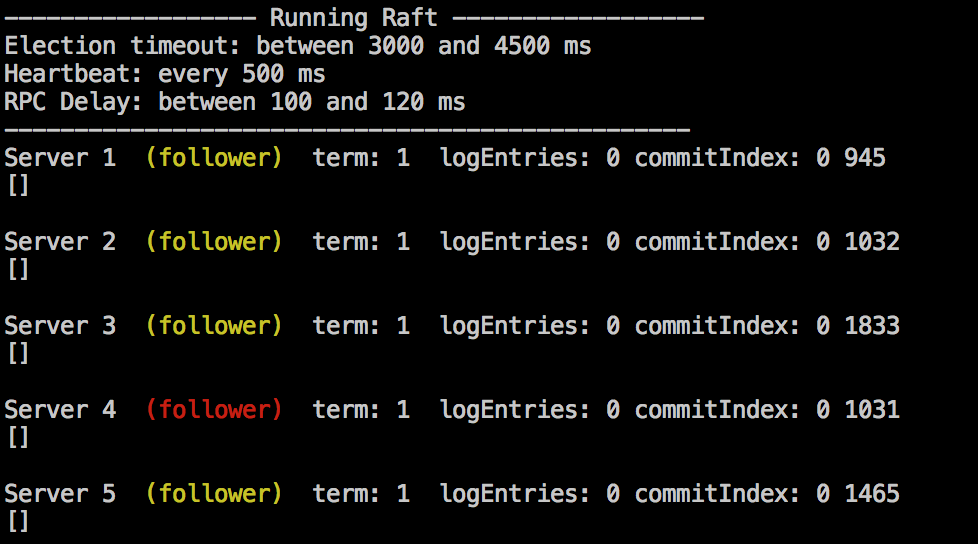
\includegraphics[scale = 0.5]{screenshot-coming-leader-election}
\caption{Example run of the simulator in the state where a leader has not yet been elected.}
\label{fig:my_label}
\end{figure}